\section{Заключение}
\label{sec:conclusion}

В ходе выполнения курсовой работы был проведен комплексный анализ данных RTB-аукционов на основе открытого датасета iPinYou. Был спроектирован и реализован полный цикл обработки данных: от очистки и нормализации сырых логов до развертывания аналитического хранилища на базе колоночной СУБД ClickHouse и построения интерактивного дашборда в Yandex DataLens. Результаты работы позволяют наглядно оценивать эффективность рекламных кампаний и исследовать факторы, влияющие на ключевые метрики (CTR, CVR, CPM).

\subsection{Описание выполненных задач}

Во время написания работы были решены все поставленные задачи:

\begin{itemize}
    \item \textbf{Проведен описательный обзор набора данных iPinYou и основных сущностей логов.} Результаты обзора, включая структуру таблиц и описание полей, представлены в разделе \ref{sec:dataset_description} (Таблицы \ref{tab:bidding_log_format}, \ref{tab:imp_clck_conv_log_format}, \ref{tab:advertiser_category}).
    \item \textbf{Выполнен расчёт и интерпретация ключевых показателей рекламных кампаний.} Метрики CPM, CTR, CVR, eCPC, eCPA рассчитаны и визуализированы на первой вкладке дашборда (Рисунки \ref{fig:tab1_kpi}, \ref{fig:tab1_trends}, \ref{fig:tab1_stats}).
    \item \textbf{Построена RTB-воронка и оценены потери на каждом этапе.} Воронка реализована в виде Advanced Chart~\cite{datalens-advanced-charts} в DataLens и представлена на Рисунке \ref{fig:tab2_funnel}.
    \item \textbf{Проанализировано влияние факторов контекста и пользователя на метрики эффективности.} Многофакторный анализ реализован на третьей вкладке дашборда (Рисунки \ref{fig:tab3_analysis1}, \ref{fig:tab3_analysis2}, \ref{fig:tab3_analysis3}).
    \item \textbf{Подготовлен пайплайн предобработки данных в Python.} Описание процесса очистки и обогащения данных приведено в подразделе \ref{subsec:data_preprocessing}, полный исходный код представлен в \href{https://github.com/wqrxssq/CourseWork}{GitHub репозитории}.
    \item \textbf{Развернута база данных и реализованы оптимизации.} Обоснование выбора ClickHouse, развертывание СУБД, ключевые архитектурные решения и процесс денормализации описаны в разделе \ref{sec:data_preparation}. DDL-определения схем доступны в \href{https://github.com/wqrxssq/CourseWork}{репозитории GitHub}. Стоит отметить, что изначальная задача развертывания базы данных в облаке была скорректирована: в связи с отсутствием гранта на Yandex Cloud, ClickHouse был развернут локально. Тем не менее, суть задачи по созданию аналитического хранилища, доступности данных и оптимизации запросов была полностью выполнена.
    \item \textbf{Построен дашборд в Yandex DataLens.} Процесс проектирования описан в разделе \ref{sec:dashboard_design}, а итоговые визуализации представлены в подразделе \ref{subsec:dashboard_visualizations}. Сам дашборд доступен по \href{https://datalens.yandex/ekzq1ggrjl24y}{ссылке}.
    \item \textbf{Пройден курс по Yandex DataLens.} В рамках освоения инструмента визуализации был успешно пройден курс, сертификат о прохождении которого представлен в \hyperref[sec:appendix]{Приложении}.
\end{itemize}

\subsection{Описание интерактивной визуализации}
\label{subsec:dashboard_visualizations}

Разработанный дашборд состоит из трех логических вкладок, решающих различные аналитические задачи. Для удобства анализа на всех вкладках предусмотрена единая панель фильтров, включающая стандартные селекторы: платформа (ОС), браузер, рекламодатель и диапазон дат. Селектор дат, в частности, позволяет фильтровать данные по сезонам соревнования (сезон 2 и сезон 3).

На Рисунках \ref{fig:tab1_kpi}, \ref{fig:tab1_trends} и \ref{fig:tab1_stats} представлена первая вкладка «Эффективность рекламы». На Рисунке \ref{fig:tab1_kpi} отображены ключевые показатели (KPI) в виде индикаторов со спарклайнами, показывающими динамику CTR, CVR, CPM, а также общие затраты бюджета, eCPC и eCPA. Рисунок \ref{fig:tab1_trends} демонстрирует тренды вовлеченности и конверсии с наложенным скользящим средним, а также распределение бюджета и кликов по топ-рекламодателям. Из графиков видно, что рекламодатель «International e-commerce» расходует наибольший бюджет, однако по объему кликов лидирует «Chinese vertical e-commerce». Рисунок \ref{fig:tab1_stats} содержит сводную таблицу со статистикой по всем рекламодателям, позволяющую детально сравнить их эффективность.

\begin{figure}[htbp]
    \centering
    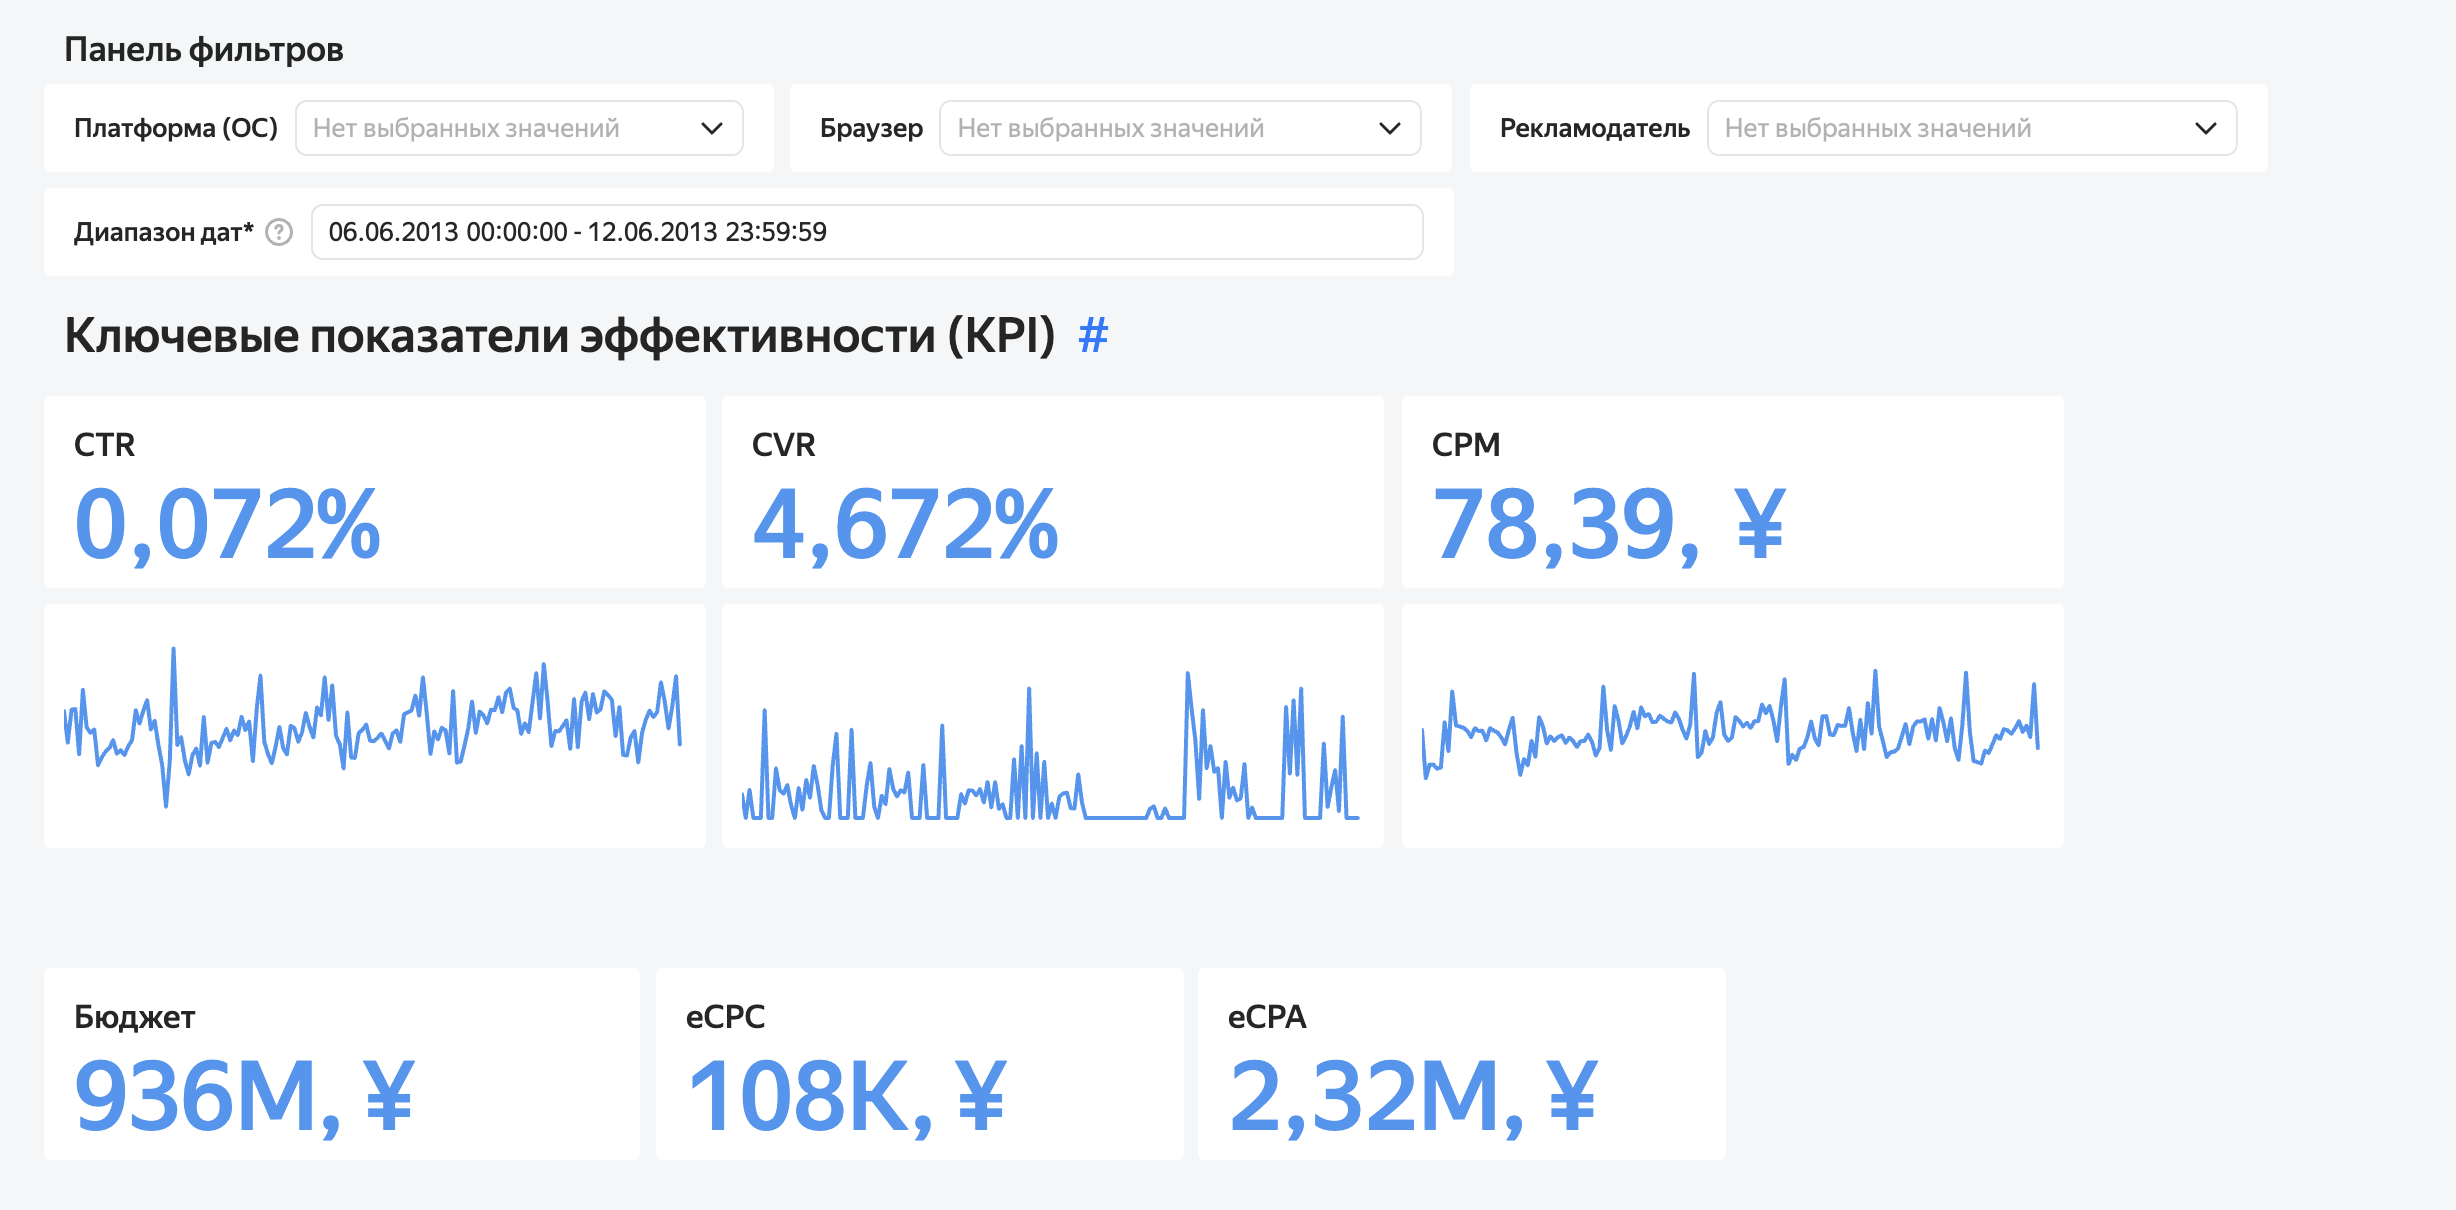
\includegraphics[width=0.95\textwidth]{images/tab1_kpi_1.png}
    \caption{Вкладка 1: Ключевые показатели эффективности (KPI)}
    \label{fig:tab1_kpi}
\end{figure}

\begin{figure}[htbp]
    \centering
    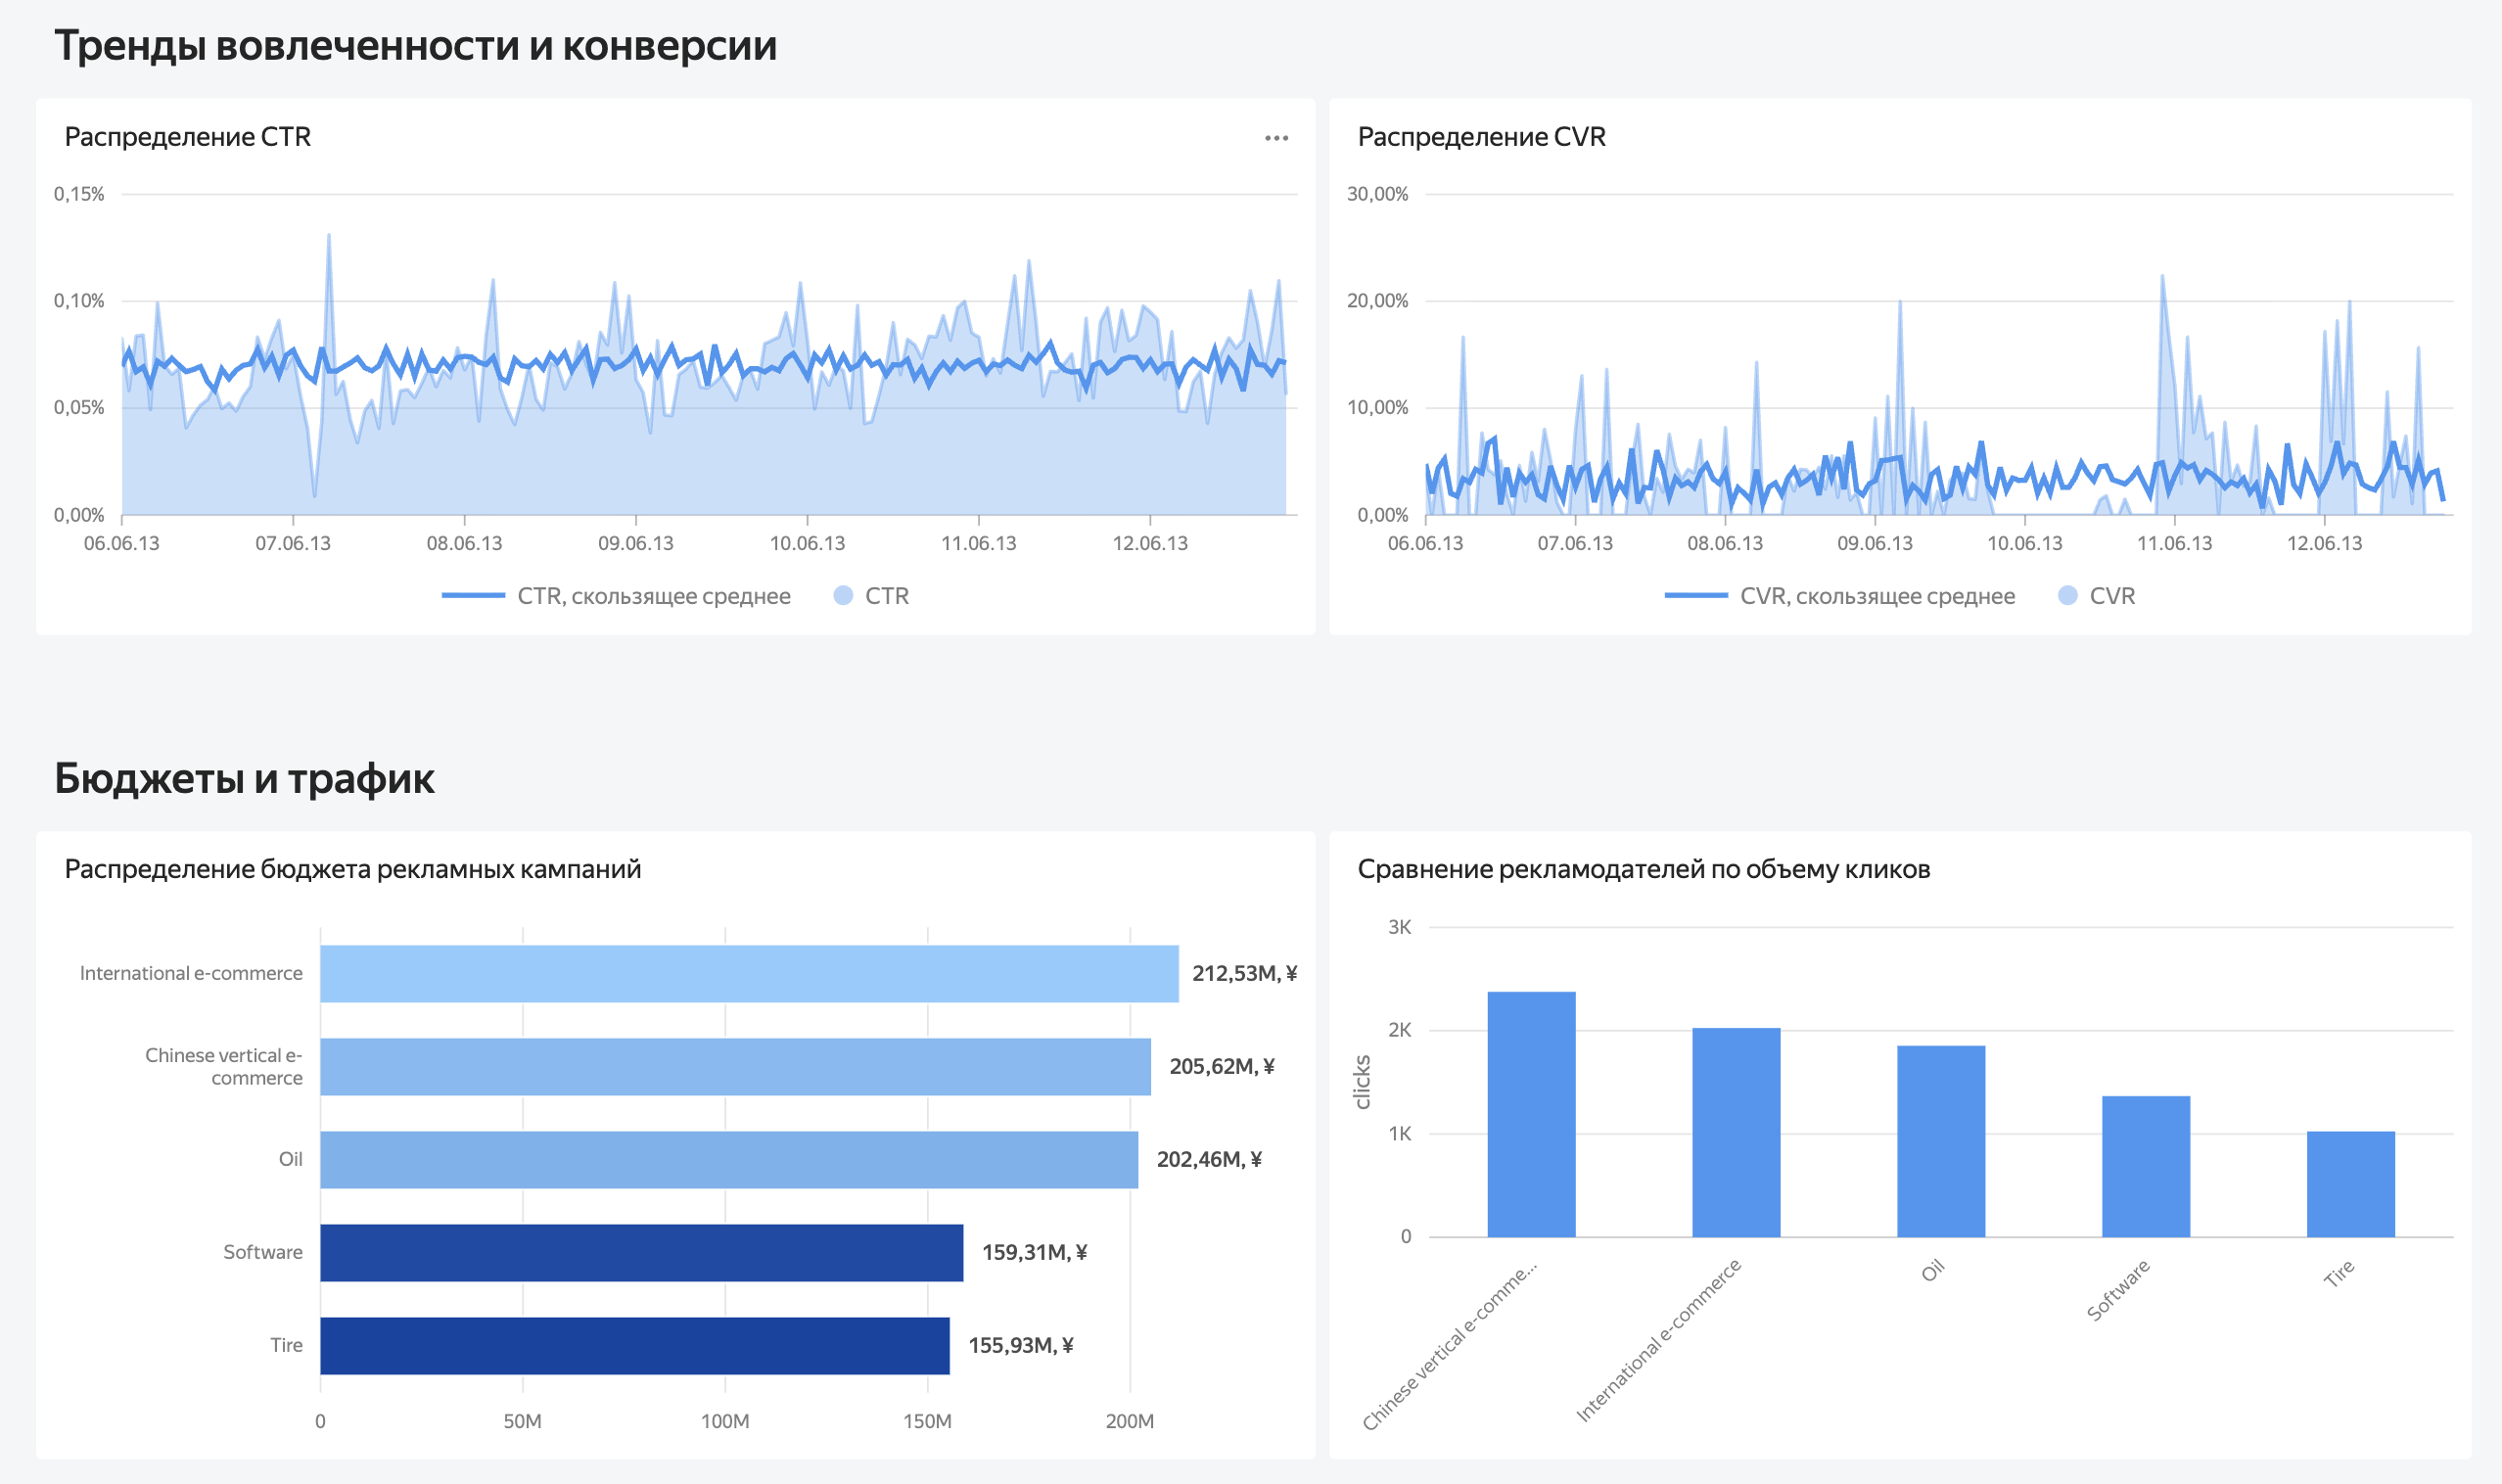
\includegraphics[width=0.95\textwidth]{images/tab1_trends_and_budgets_2.png}
    \caption{Вкладка 1: Тренды вовлеченности и распределение бюджетов}
    \label{fig:tab1_trends}
\end{figure}

\begin{figure}[htbp]
    \centering
    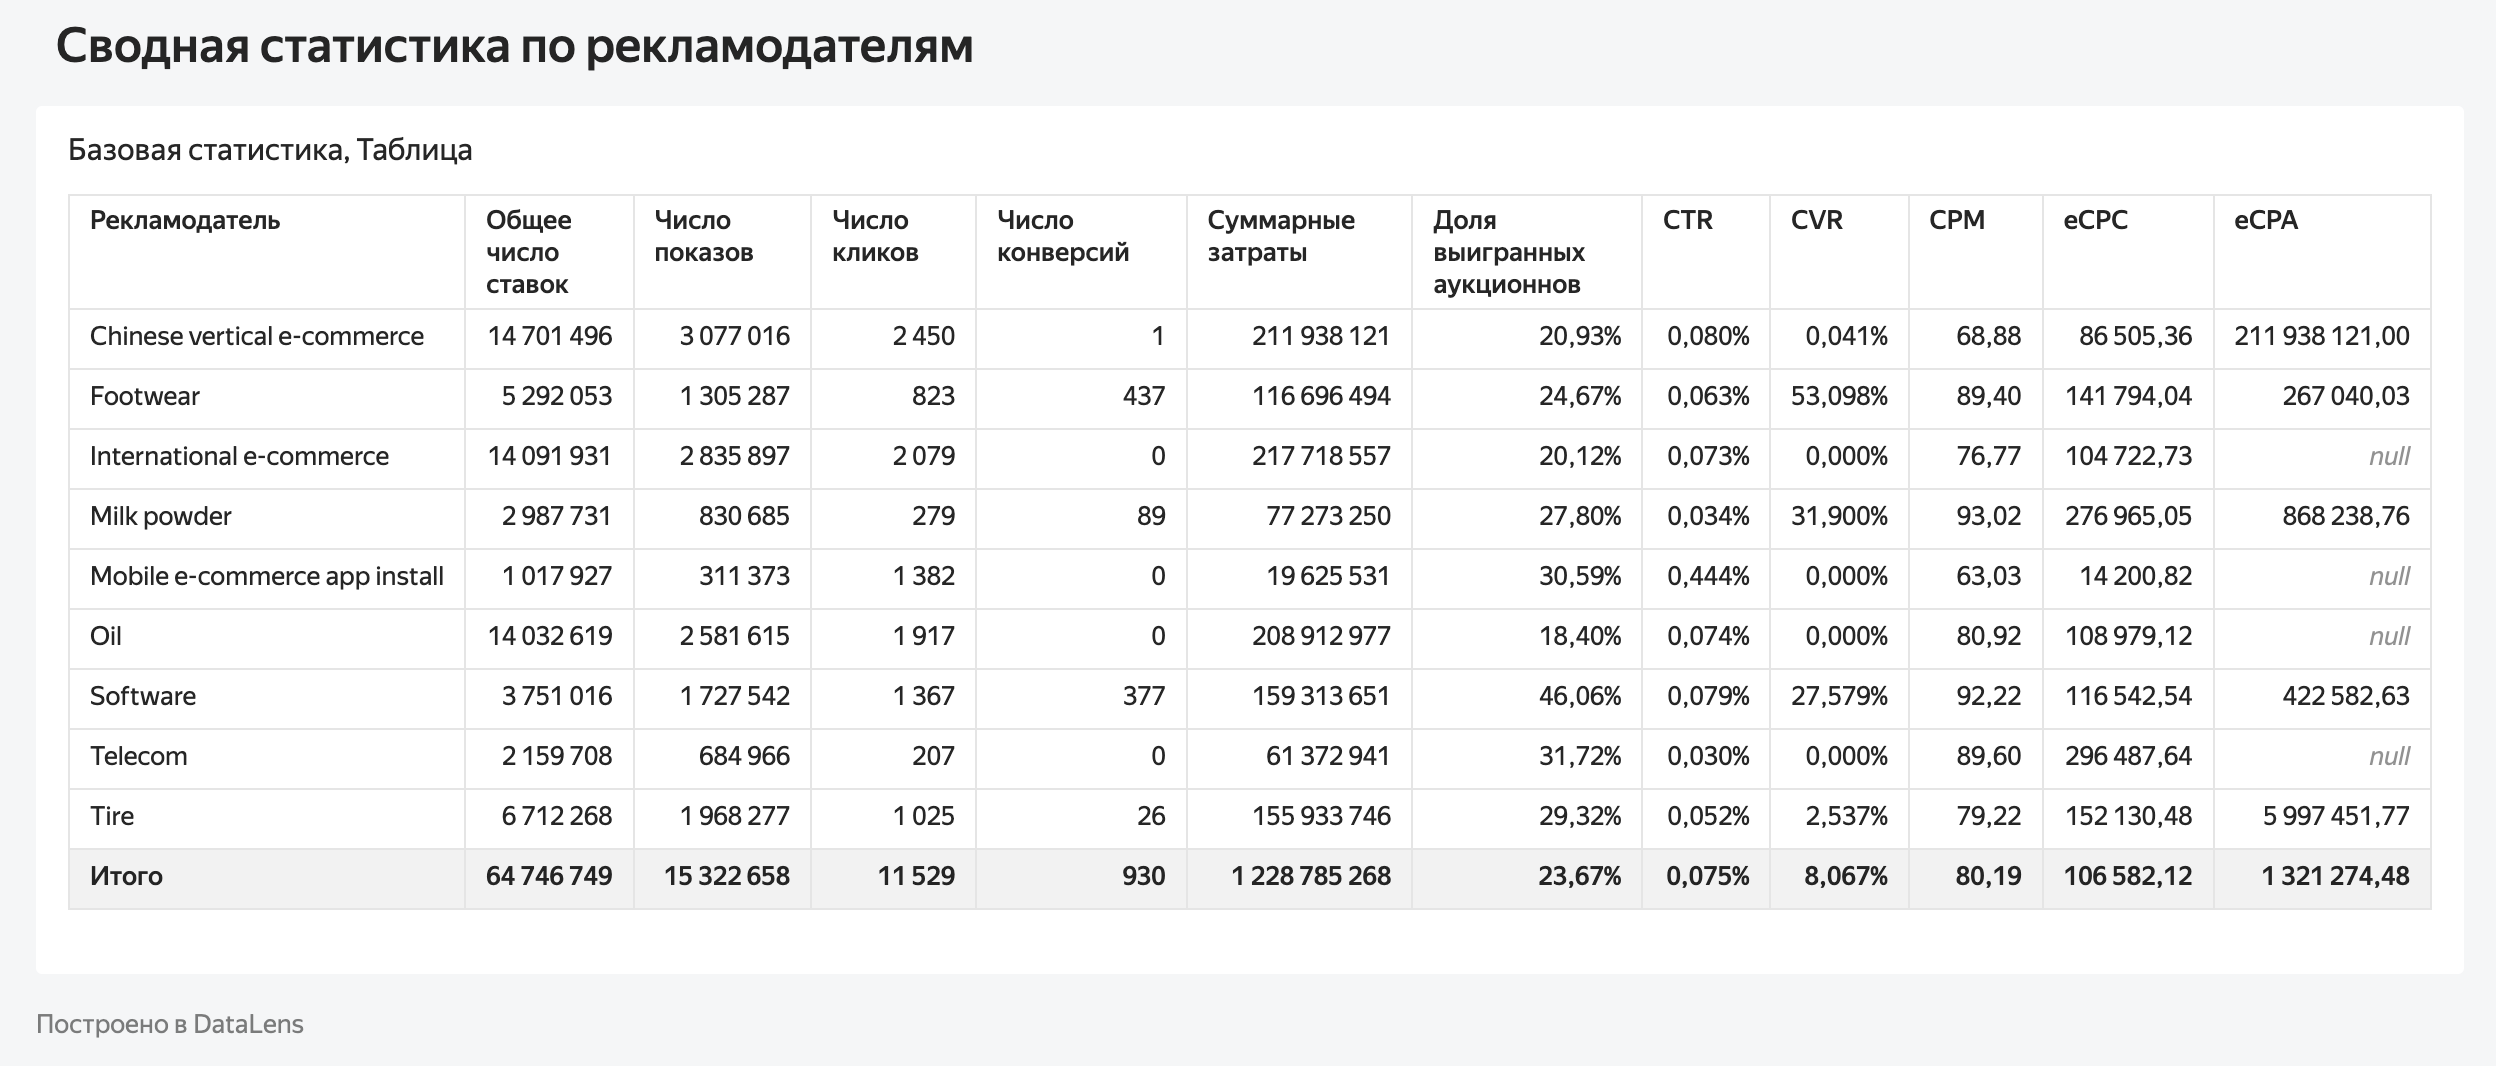
\includegraphics[width=0.95\textwidth]{images/tab1_statistics_3.png}
    \caption{Вкладка 1: Сводная статистика по рекламодателям}
    \label{fig:tab1_stats}
\end{figure}
\newpage

Вторая вкладка «EDA» (Рисунки \ref{fig:tab2_funnel}, \ref{fig:tab2_traffic1}, \ref{fig:tab2_traffic2}) посвящена разведочному анализу. На Рисунке \ref{fig:tab2_funnel} визуализирована RTB-воронка, наглядно демонстрирующая колоссальные потери трафика на каждом этапе: из 53 млн ставок лишь 22,9\% выигрывают аукцион, из показов только 0,072\% конвертируются в клики, а из кликов — 4,57\% в целевые действия. Рисунок \ref{fig:tab2_traffic1} показывает структуру трафика: преобладание ОС Windows и браузера IE/Chrome, а также распределение по регионам Китая (лидирует Guangdong), для которого предусмотрен селектор TOP-K, позволяющий гибко настраивать количество отображаемых регионов. Рисунок \ref{fig:tab2_traffic2} иллюстрирует временную динамику объема трафика в разрезе часа дня, показывая спад активности в ночные часы и пик в вечернее время. Также на этом рисунке представлена гистограмма распределения относительного спреда, характеризующая конкурентность аукциона.

\begin{figure}[htbp]
    \centering
    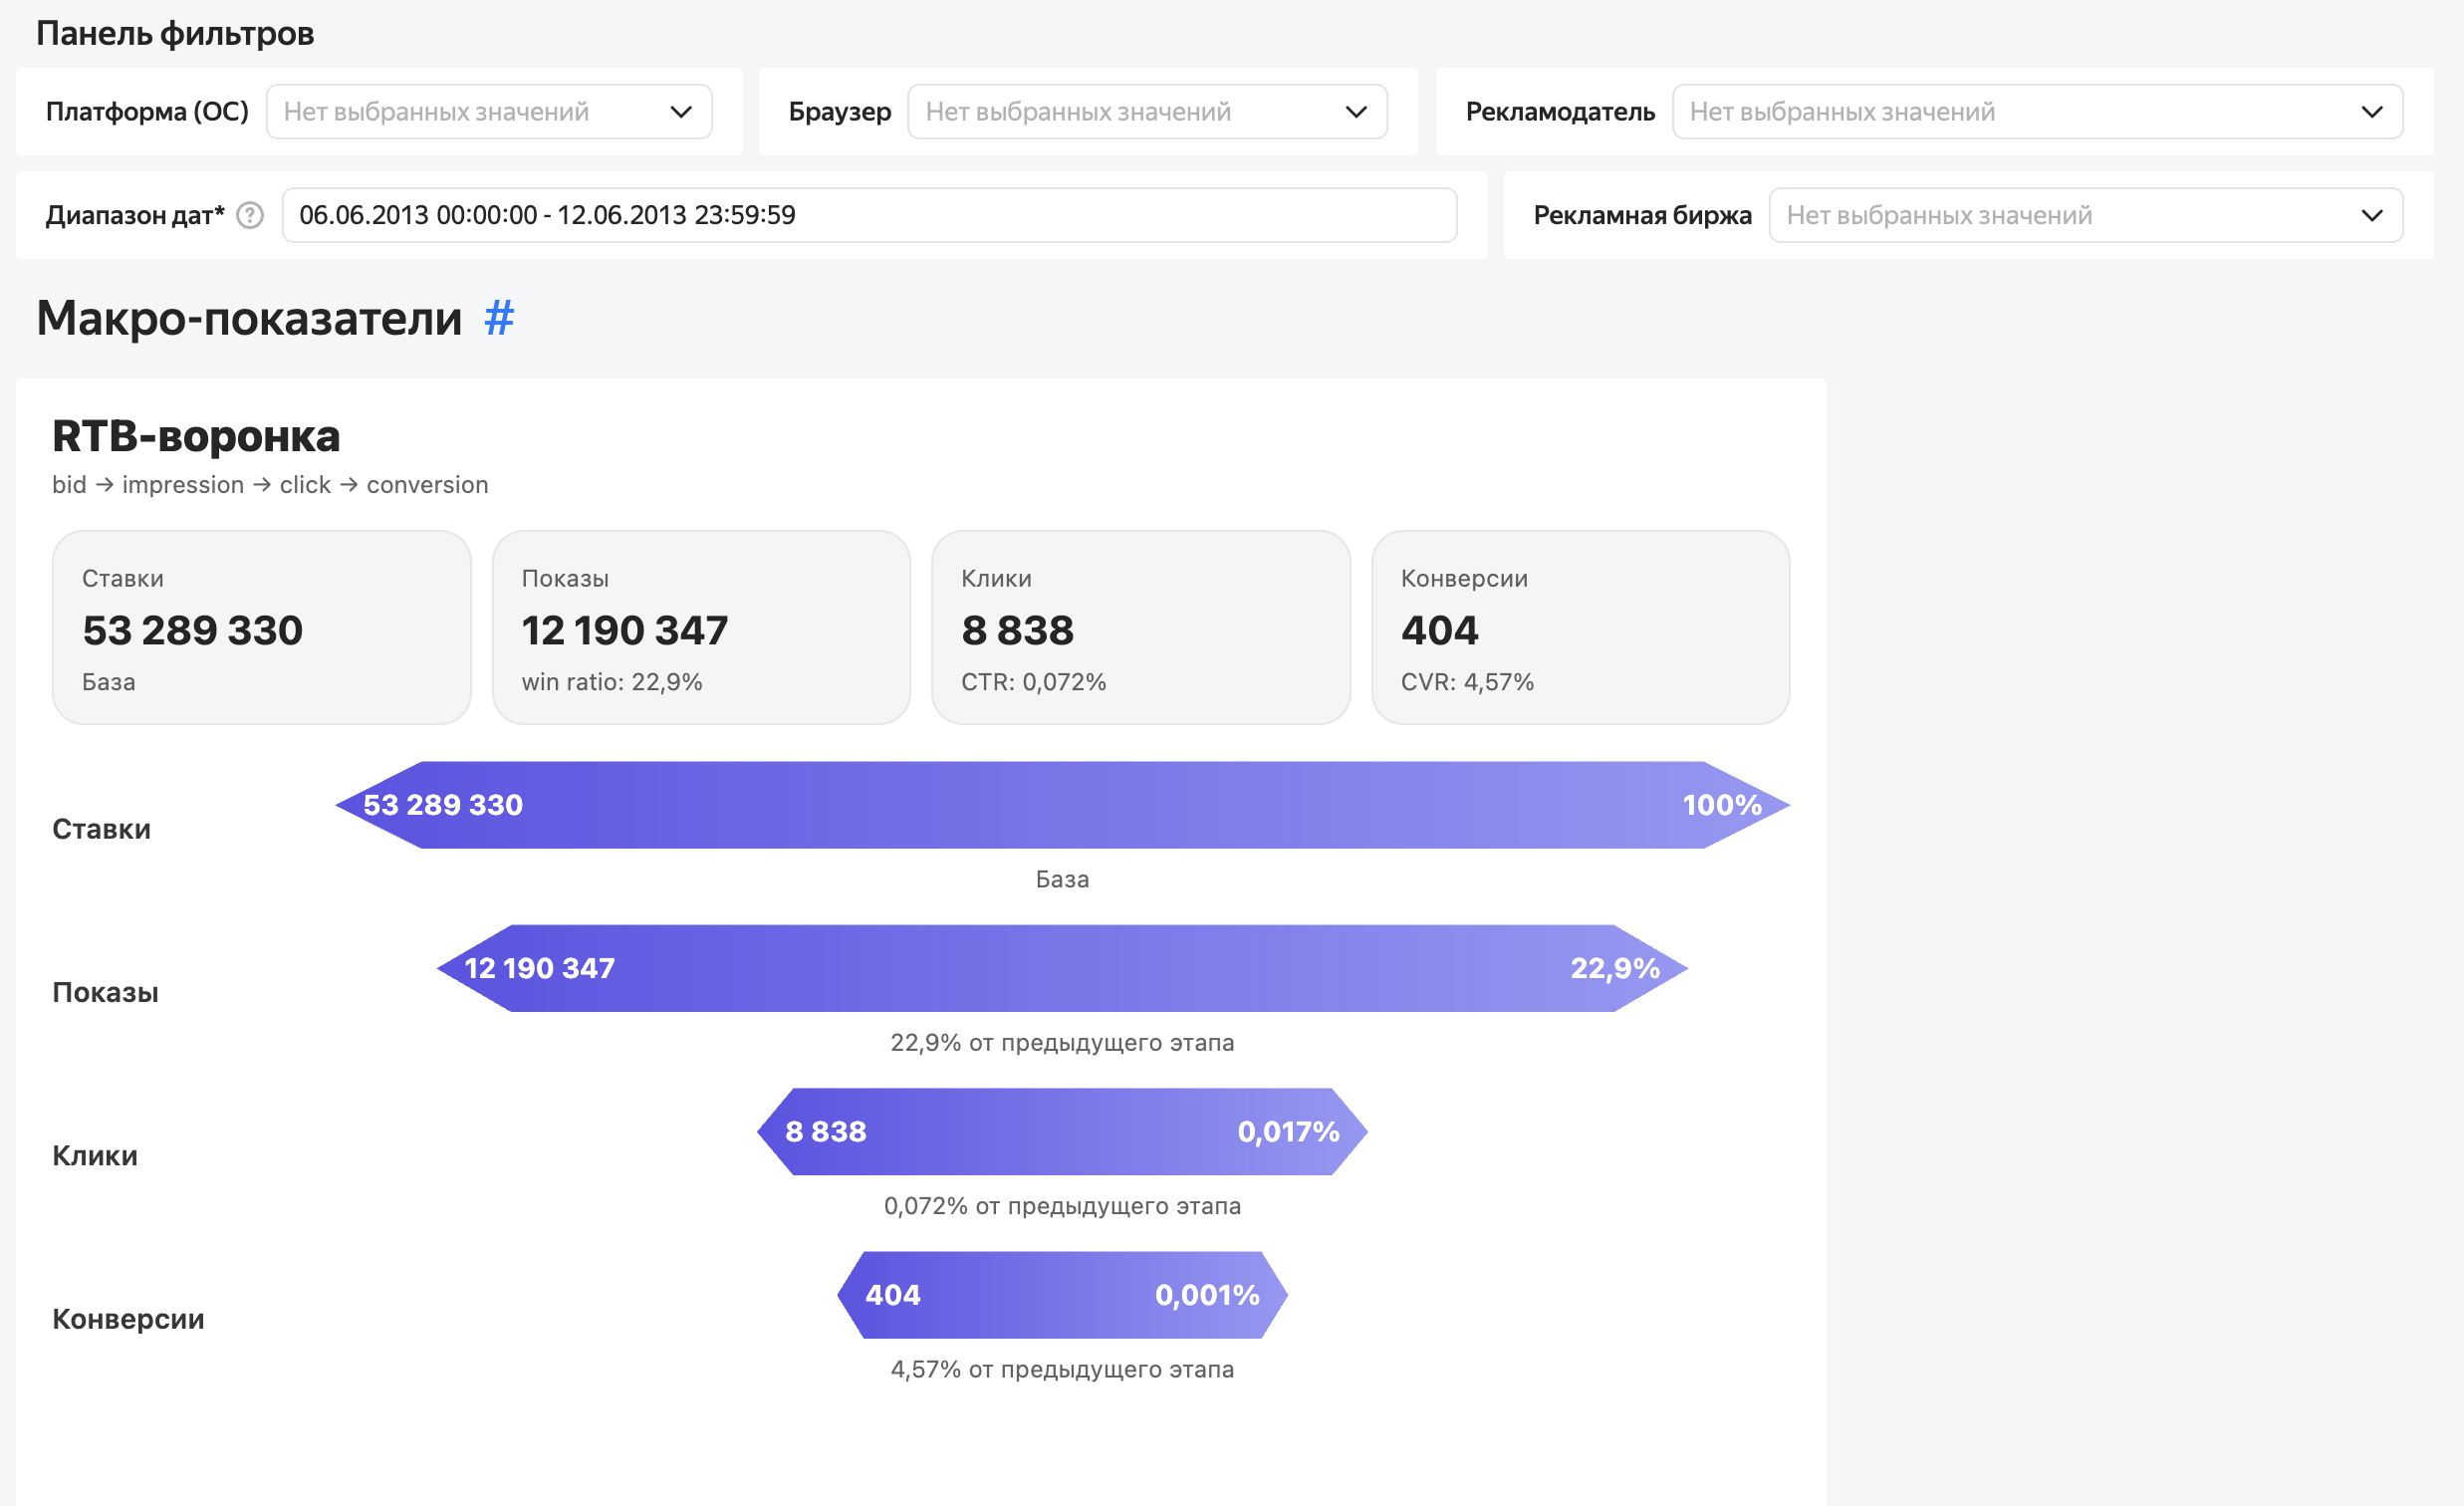
\includegraphics[width=0.95\textwidth]{images/tab2_rtb_funnel_4.png}
    \caption{Вкладка 2: RTB-воронка}
    \label{fig:tab2_funnel}
\end{figure}

\begin{figure}[htbp]
    \centering
    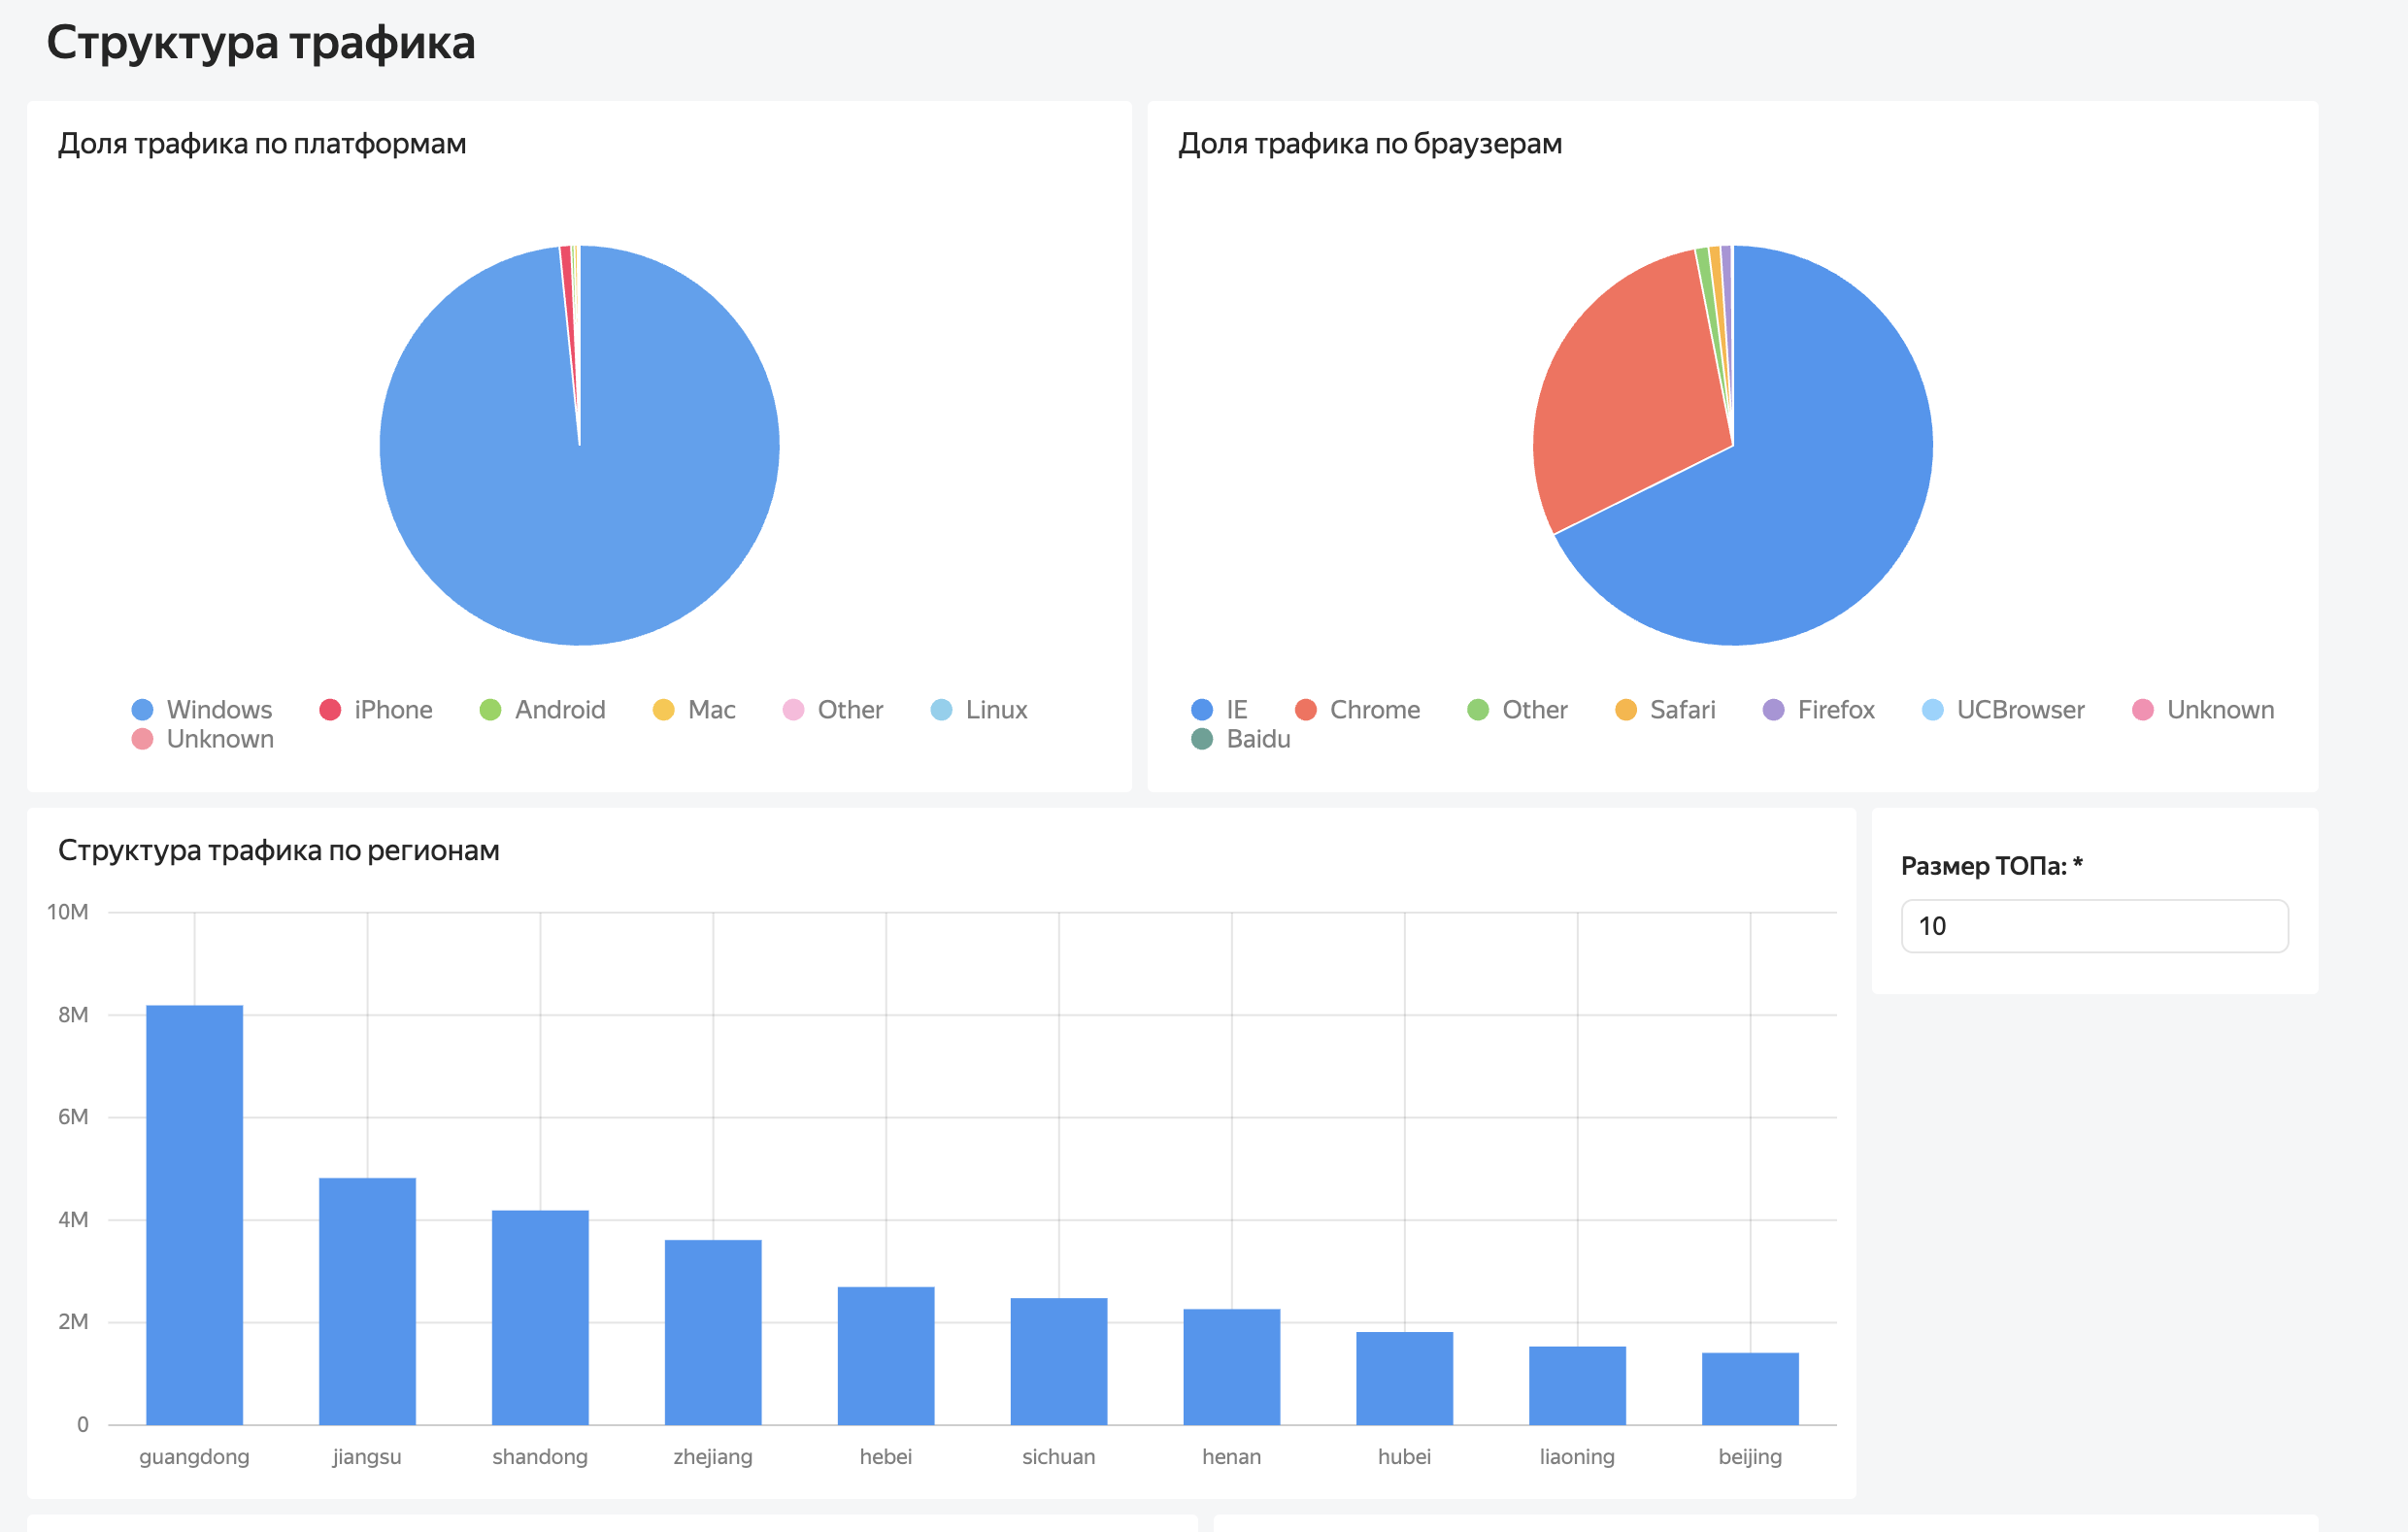
\includegraphics[width=0.95\textwidth]{images/tab2_traffic1_5.png}
    \caption{Вкладка 2: Структура трафика по платформам, браузерам и регионам}
    \label{fig:tab2_traffic1}
\end{figure}

\begin{figure}[htbp]
    \centering
    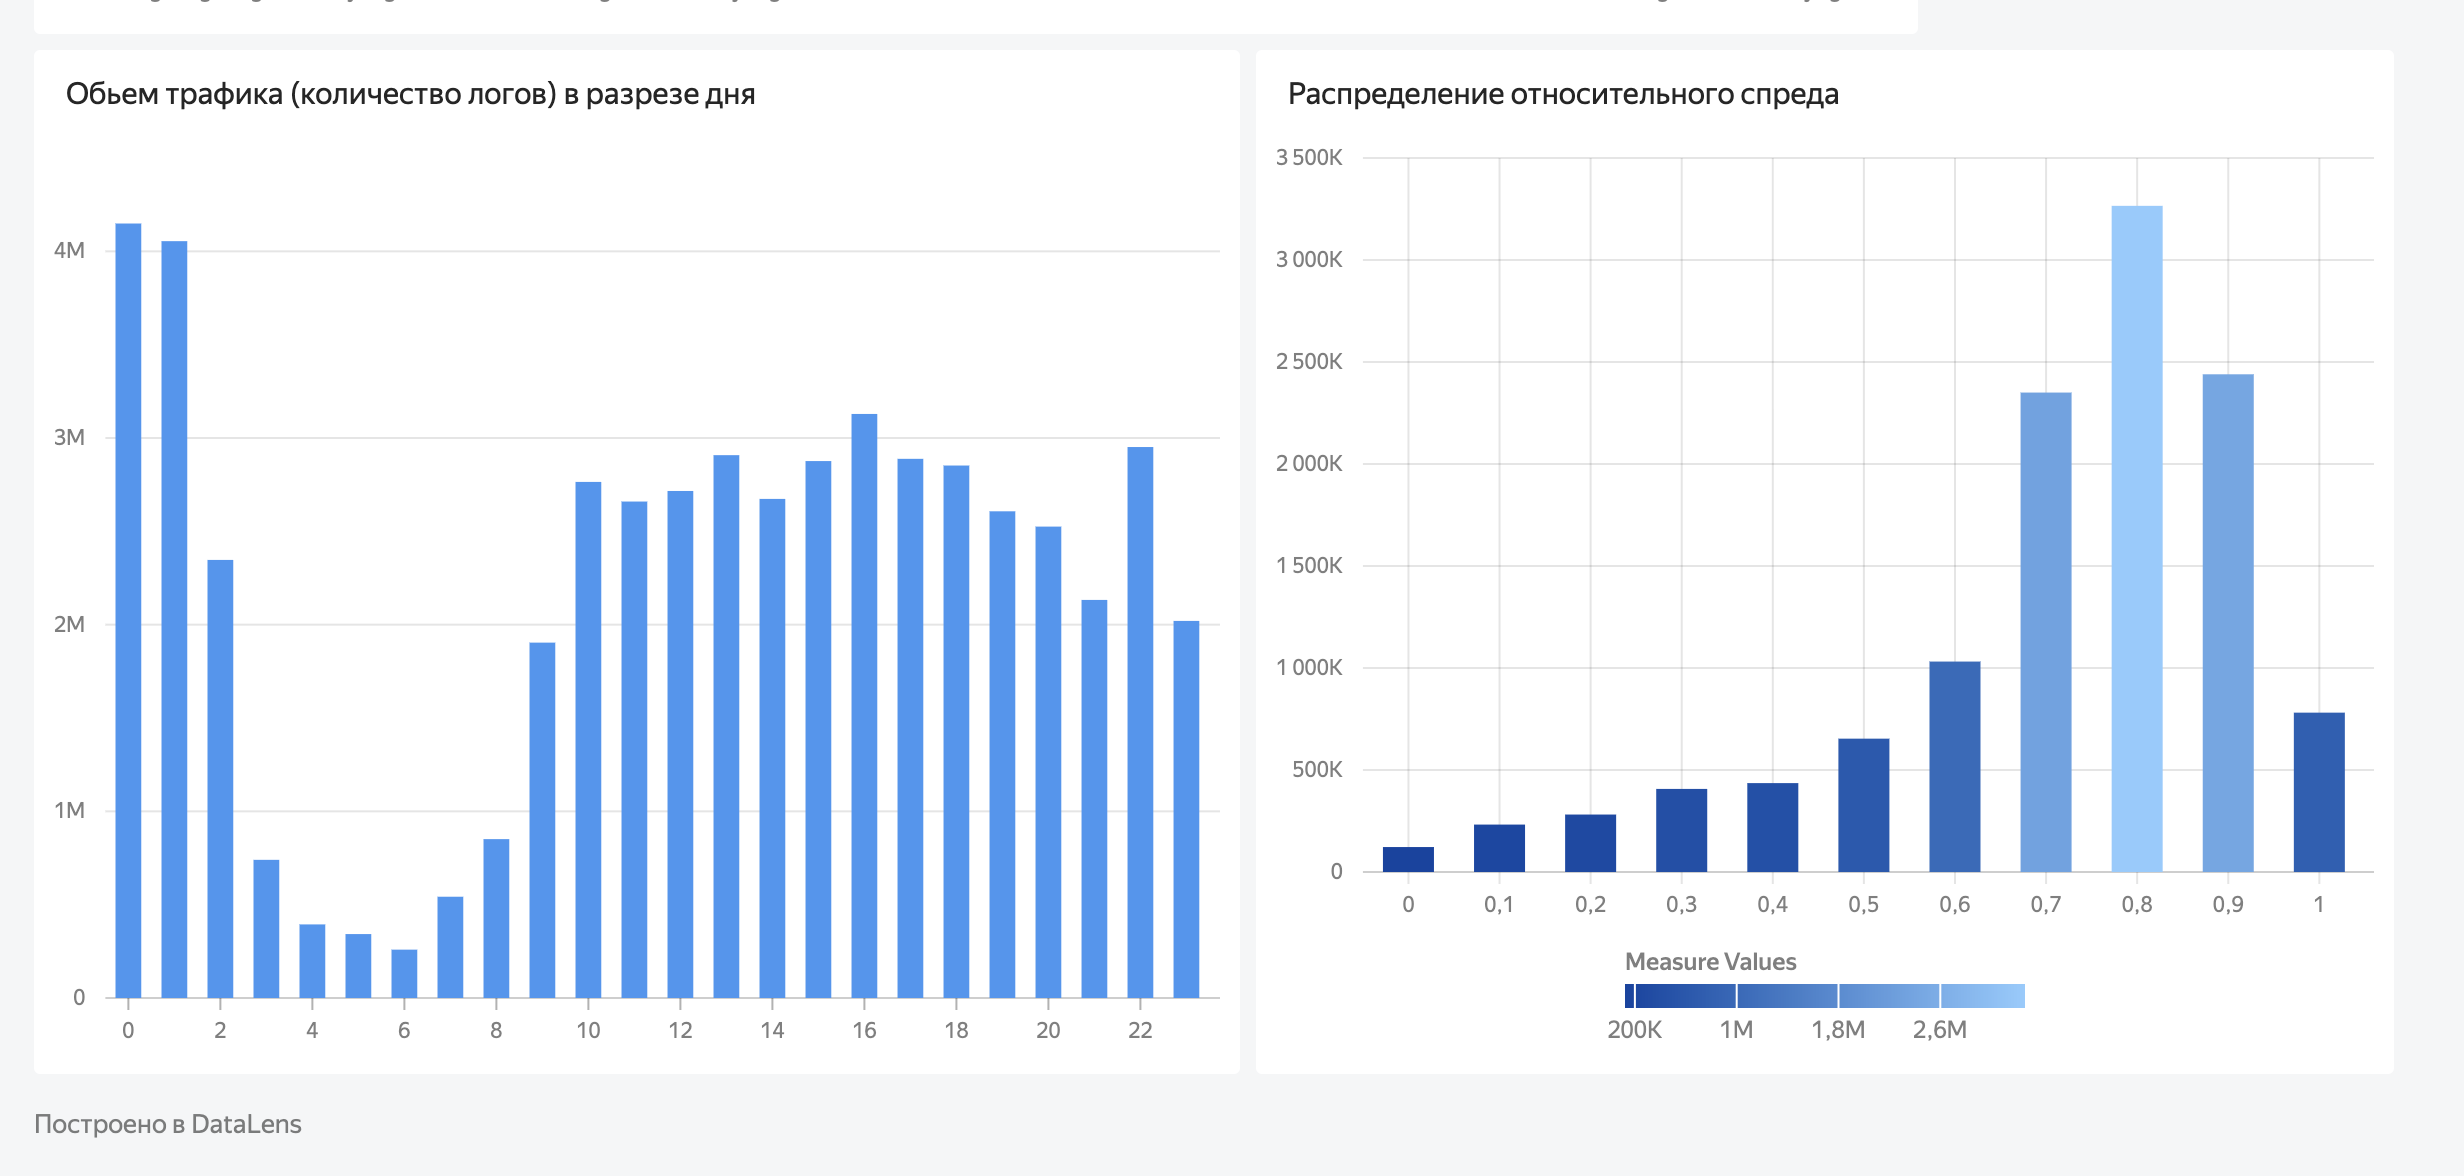
\includegraphics[width=0.95\textwidth]{images/tab2_traffic2_6.png}
    \caption{Вкладка 2: Объем трафика по часам и распределение спреда}
    \label{fig:tab2_traffic2}
\end{figure}
\newpage

Третья вкладка «Многофакторный анализ» (Рисунки \ref{fig:tab3_analysis1}, \ref{fig:tab3_analysis2}, \ref{fig:tab3_analysis3}) позволяет исследовать влияние различных параметров на выбранную метрику (в данном примере — CTR). Уникальность данной вкладки заключается в ее интерактивности: благодаря селектору выбора анализируемой метрики, пользователь может проверять огромное количество гипотез, используя всего 7 динамически перестраиваемых графиков в зависимости от выбранной метрики (столбчатые диаграммы для формата, места размещения, платформы и браузера, диаграмму рассеяния для размера креатива, а также линейные графики для временной динамики по дням недели и часам). Рисунок \ref{fig:tab3_analysis1} показывает, что всплывающий формат рекламы (Pop) имеет значительно более высокий CTR по сравнению с фиксированным (Fixed), а диаграмма рассеяния демонстрирует линейную зависимость метрики от размера креатива. На Рисунке \ref{fig:tab3_analysis2} видно влияние контекста: размещение FirstView показывает наилучший результат, а мобильные платформы (Android, iPhone) демонстрируют более высокий CTR по сравнению с десктопными. Рисунок \ref{fig:tab3_analysis3} отражает временную динамику метрики, показывая зависимость от дня недели и часа.

\begin{figure}[htbp]
    \centering
    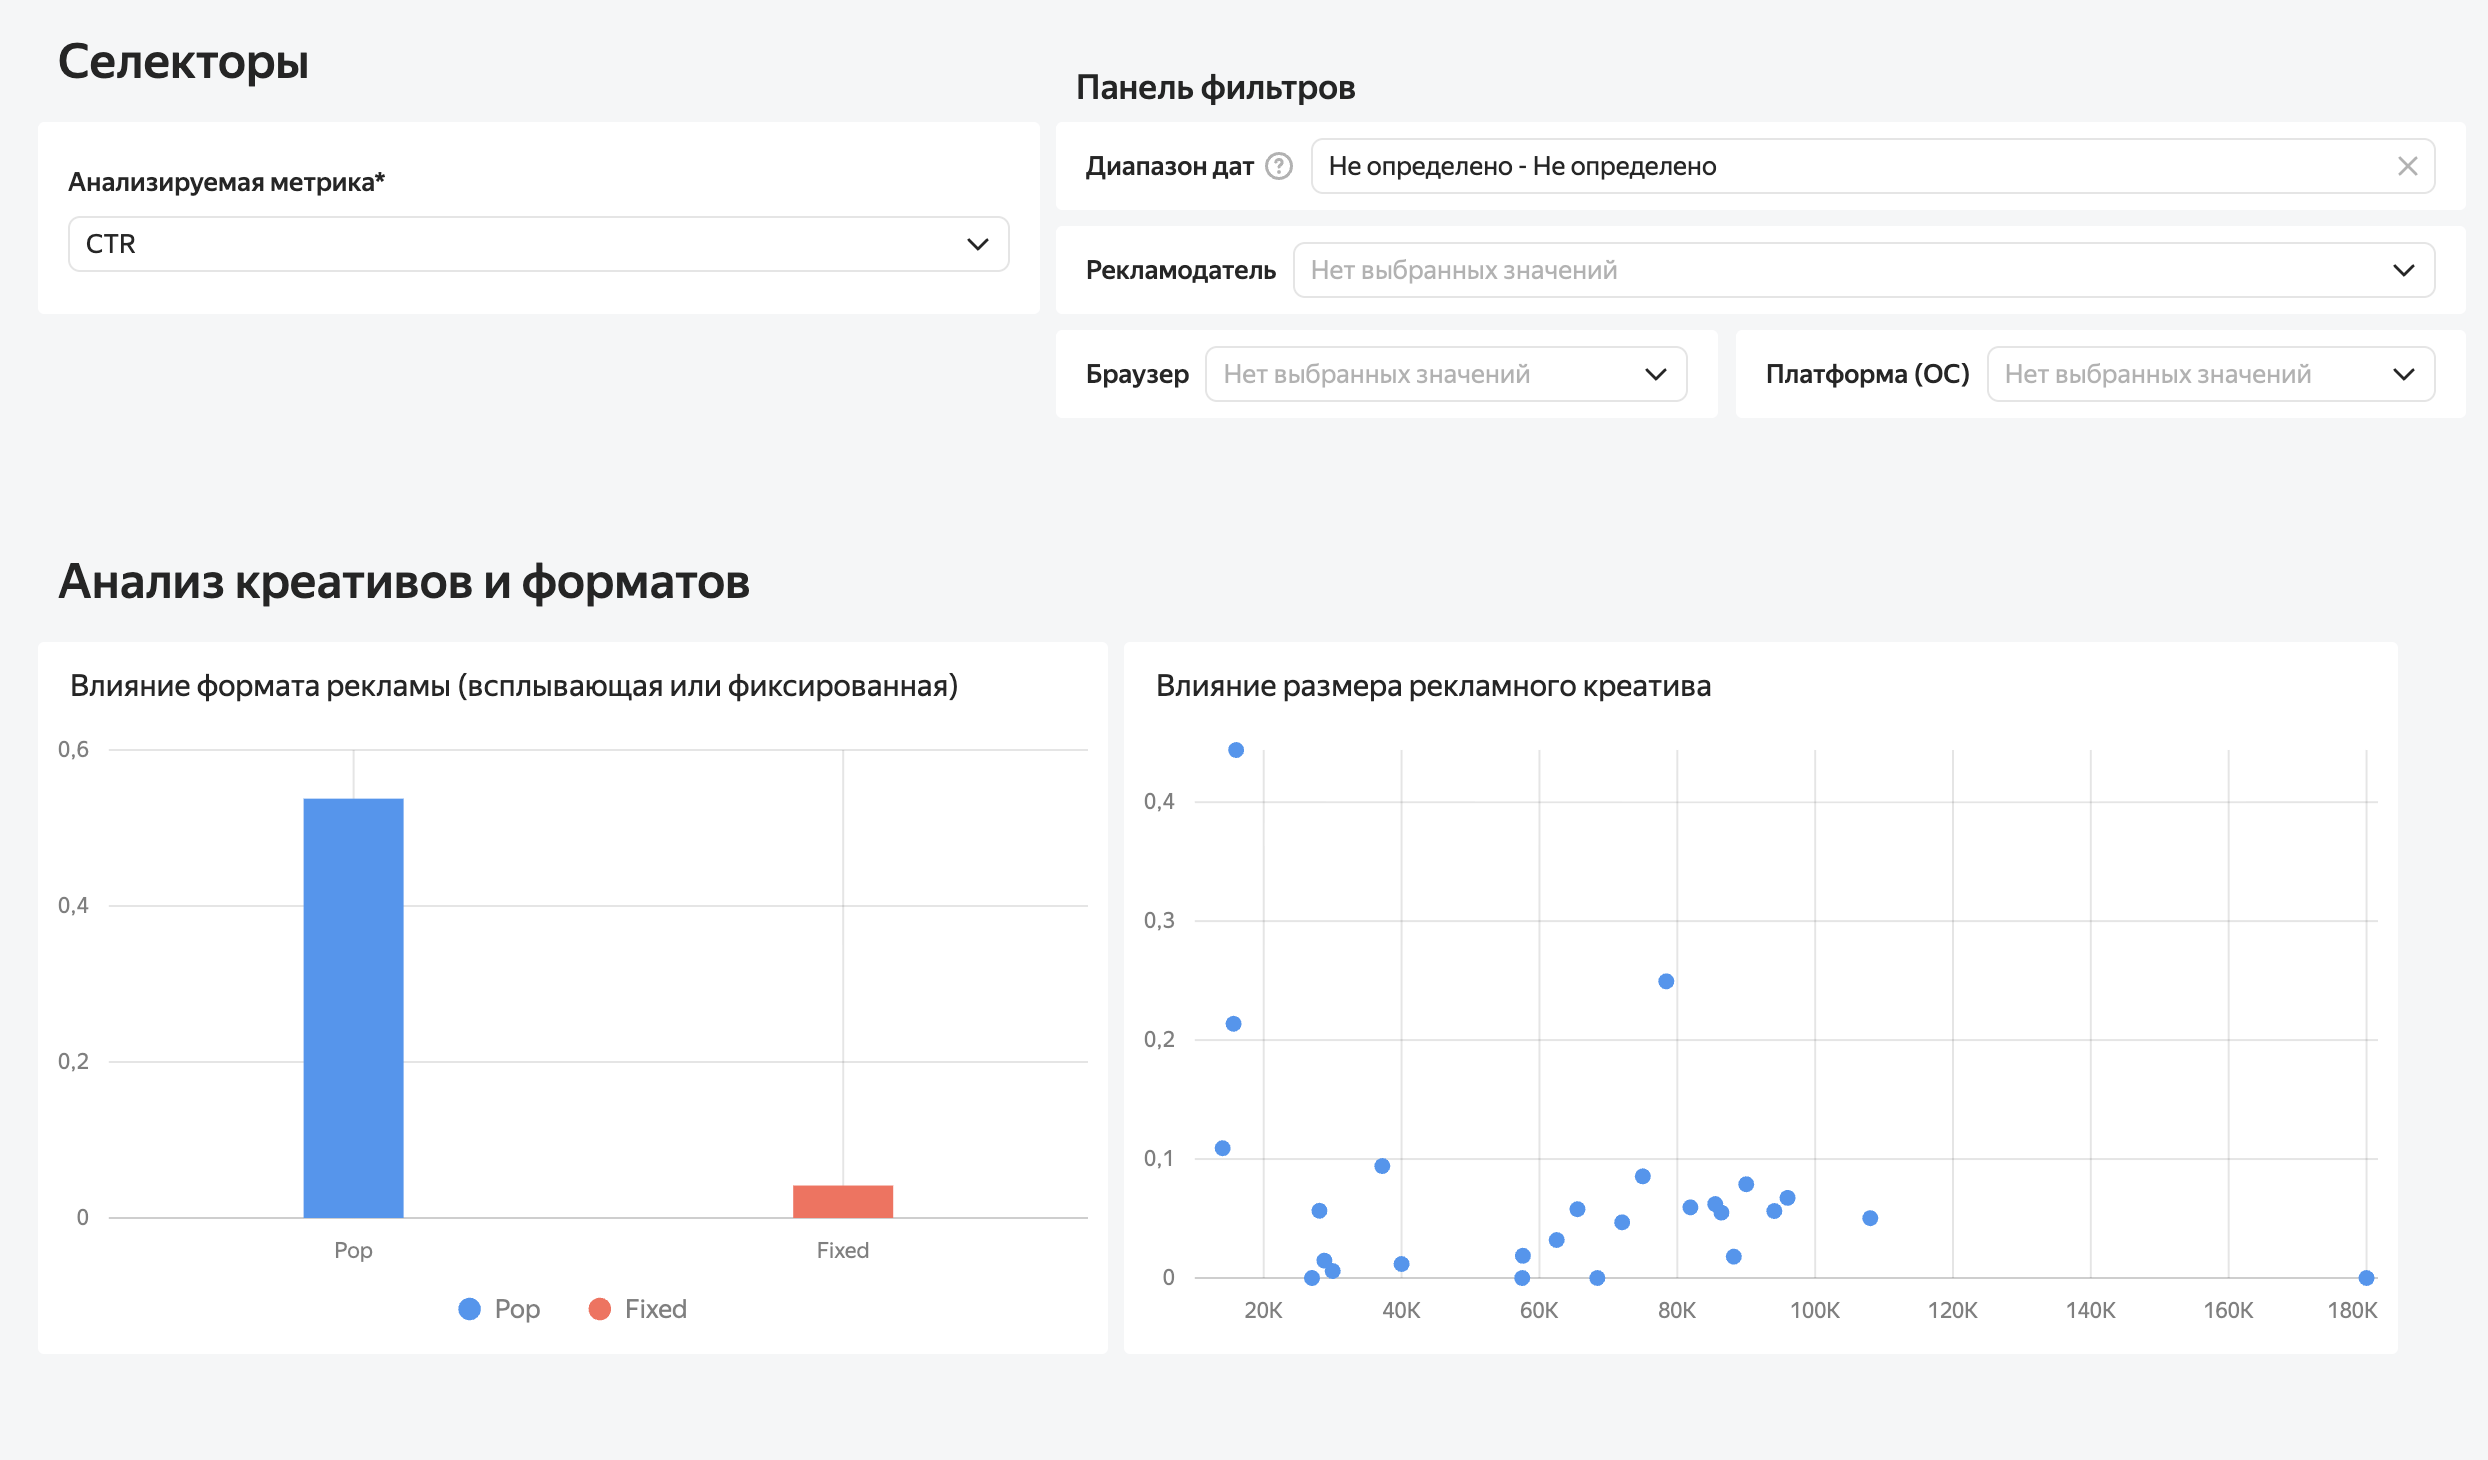
\includegraphics[width=0.95\textwidth]{images/tab3_anylisis_7.png}
    \caption{Вкладка 3: Влияние формата и размера креатива на метрику}
    \label{fig:tab3_analysis1}
\end{figure}

\begin{figure}[htbp]
    \centering
    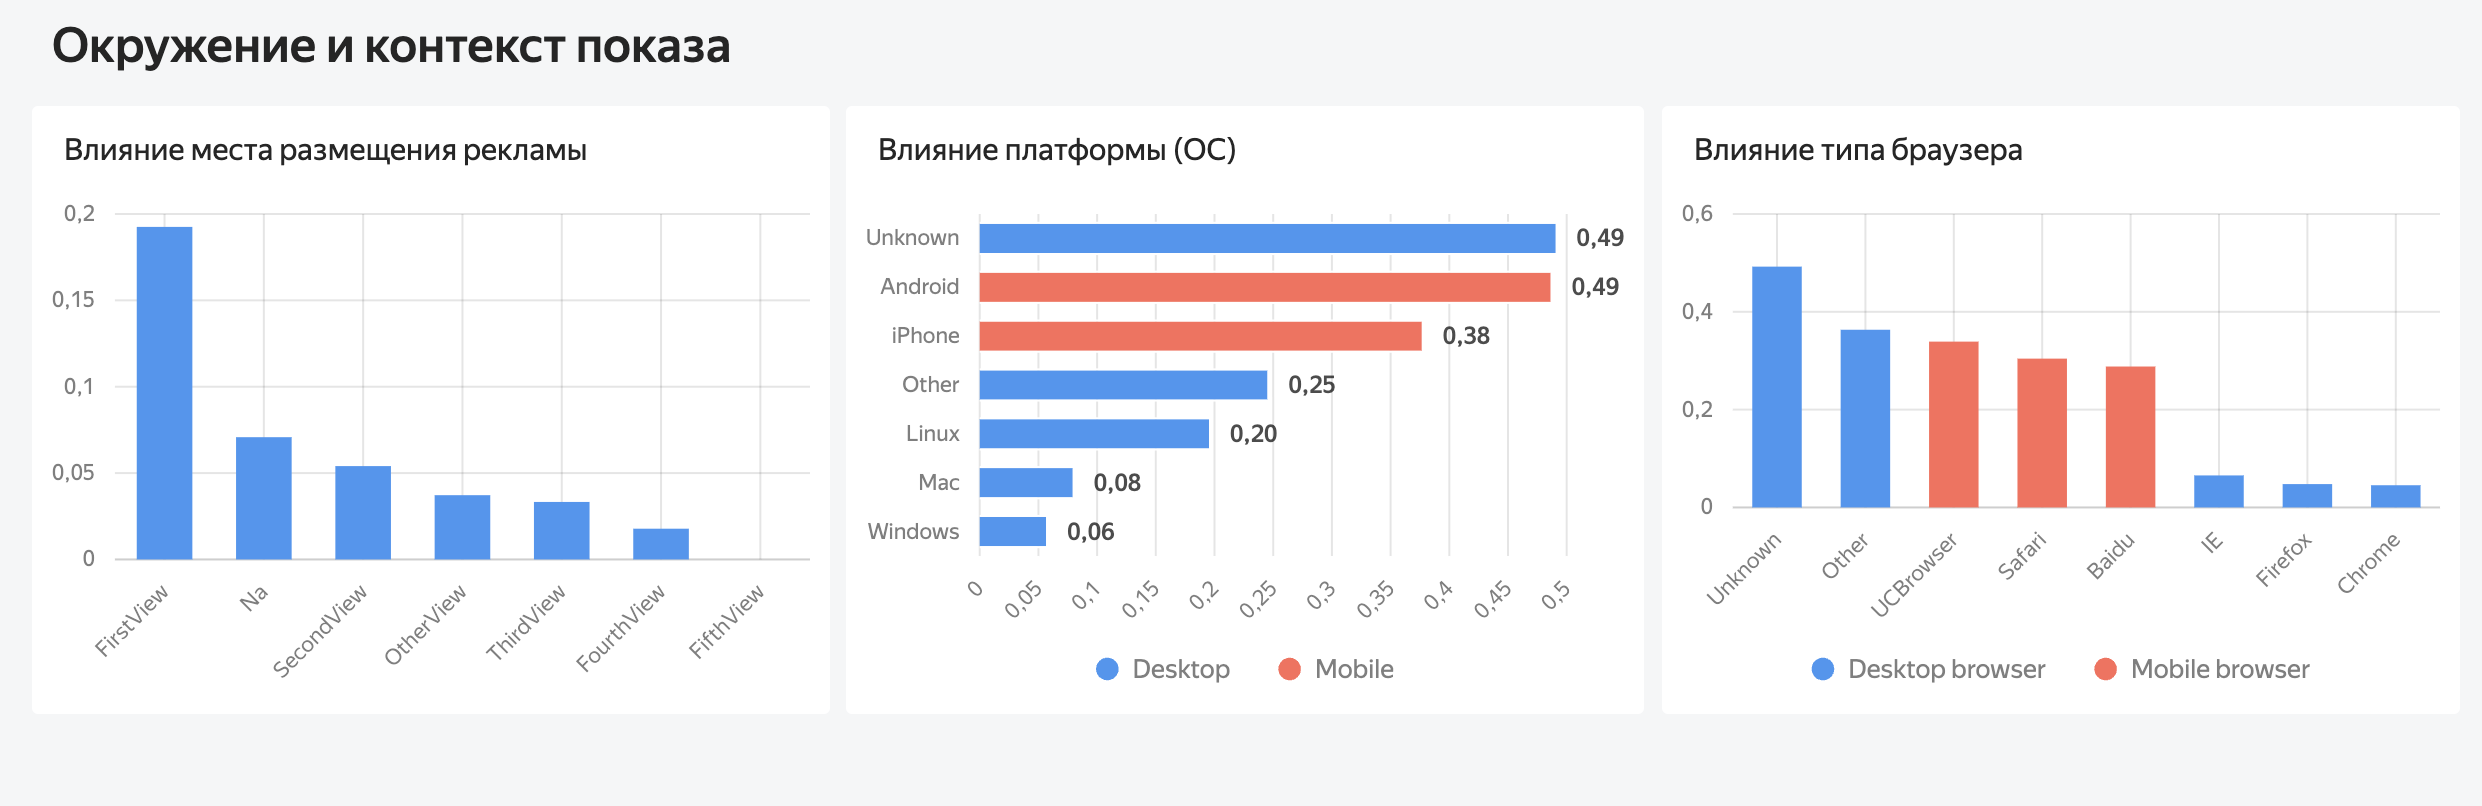
\includegraphics[width=0.95\textwidth]{images/tab3_analysis2_8.png}
    \caption{Вкладка 3: Влияние места размещения, платформы и браузера}
    \label{fig:tab3_analysis2}
\end{figure}

\begin{figure}[htbp]
    \centering
    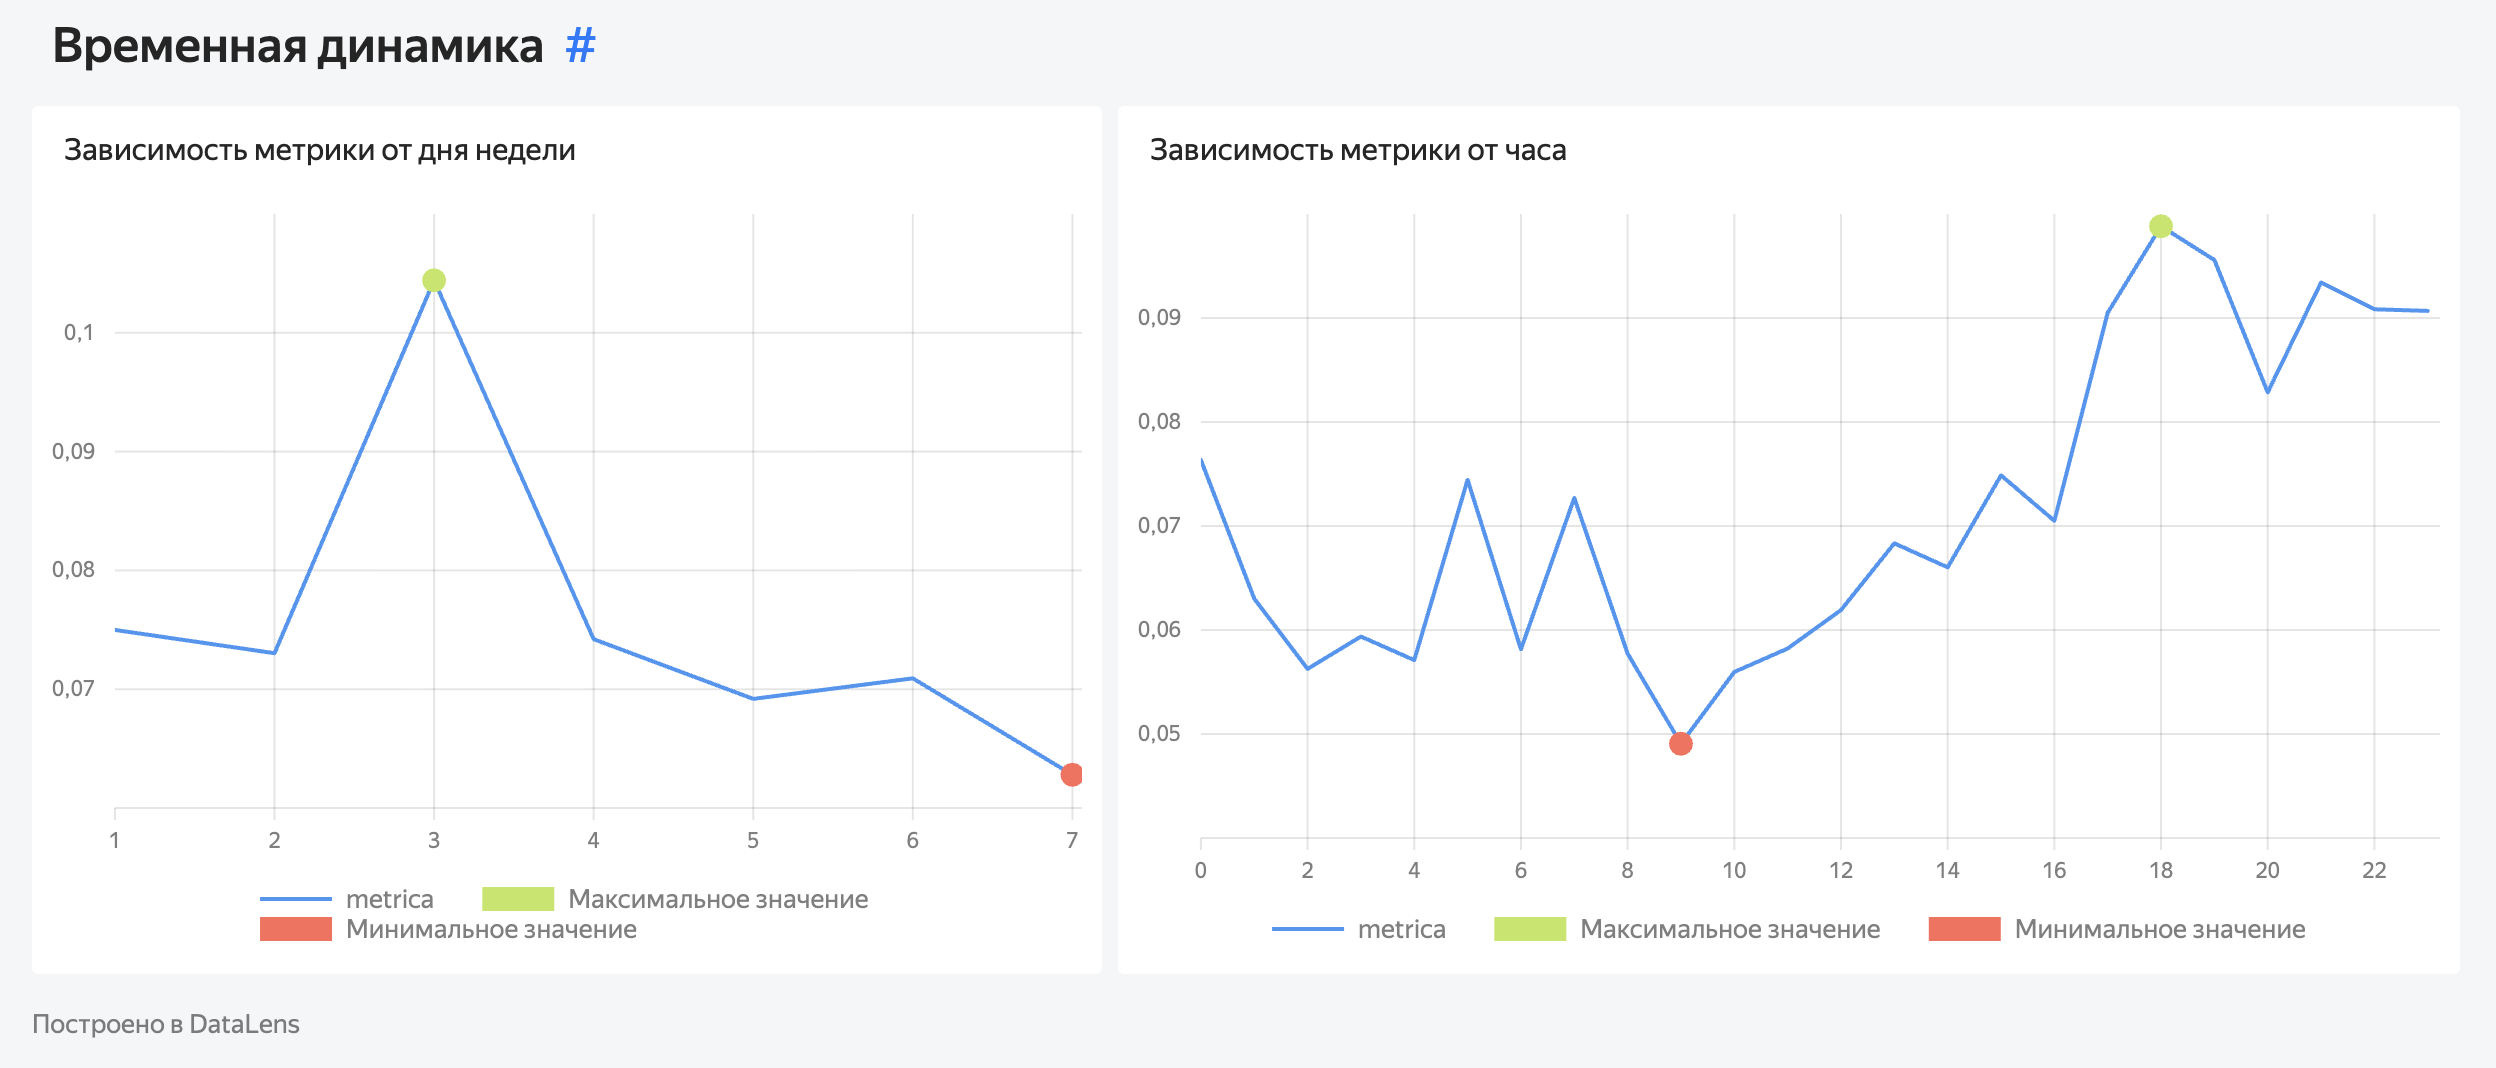
\includegraphics[width=0.95\textwidth]{images/tab3_analysis3_9.png}
    \caption{Вкладка 3: Временная динамика метрики}
    \label{fig:tab3_analysis3}
\end{figure}

\subsection{Ответ на основной вопрос работы}

Основным вопросом исследования являлось определение масштаба потерь на каждом этапе RTB-воронки и выявление факторов, оказывающих наиболее сильное влияние на эффективность рекламных кампаний.

Анализ воронки показал обьем потерь на каждом этапе: из всех сделанных ставок выигрывают около 22\%, из показов в клики переходит всего 0,072\%, а из кликов в конверсии —- около 4,5-5\%. В итоге до целевого действия доходит порядка 0,001\% от начального числа ставок. Это подчеркивает сложность задачи оптимизации ставок: алгоритмам DSP приходится обрабатывать десятки миллионов строк логов ради получения сотен конверсий, что делает критически важным правильный выбор аналитической инфраструктуры.

При анализе факторов выявилены следующие ключевые закономерности:
\begin{itemize}
    \item \textbf{Формат и размер креатива:} Всплывающие окна показывают CTR, превышающий фиксированные форматы более чем в 10 раз, при разнице в CPM всего в 2 раза. Размер креатива также линейно влияет на CTR, но также линейно увеличивает стоимость показа.
    \item \textbf{Видимость и устройство:} Размещение в первой зоне видимости увеличивает CTR в 2,7 раза по сравнению со следующей зоной при почти равном CPM. Мобильные устройства демонстрируют значительно больший CTR при примерно одинаковой цене закупки по сравнению с дектопными устройствами.
    \item \textbf{Время:} Час дня оказывает существенное влияние на долю кликов, в то время как день недели оказался достаточно слабым признаком.
    \item \textbf{Конверсия (CVR):} фиксированный формат рекламы имеет CVR в 2 раза выше, чем вспылвающий. Это вероятно говорит о том, что высокий CTR всплывающих окон во многом обьясняется случайными нажатиями, а не реальным интересом.
\end{itemize}

Важно отметить, что не существует единственно верной метрики рекламной кампании. Рекламодатель должен самостоятельно определять приоритеты (максимизация охвата, кликов или конверсий) и стратегию расхода бюджета. Разработанный дашборд на базе Yandex DataLens предоставляет необходимые методы для принятия таких аналитических решений.

\subsection{Ограничения работы}

В ходе выполнения работы был выявлен ряд ограничений:
\begin{itemize}
    \item \textbf{Сложность визуализации нестандартных чартов:} RTB-воронка потребовала использования функционала Advanced Charts в DataLens, что влечет за собой необходимость написания кода на JavaScript вместо использования UI.
    \item \textbf{Актуальность данных:} Набор данных iPinYou, несмотря на свою полноту и академическую ценность, является относительно старым. Экосистема RTB активно развивается, появляются новые форматы и алгоритмы, поэтому для подтверждения выявленных закономерностей в современных реалиях требуется анализ более свежих датасетов при сохранении аналогичного уровня детализации.
\end{itemize}

\subsection{Развитие работы}

Дальнейшее развитие проекта может осуществляться в следующих направлениях:
\begin{itemize}
    \item \textbf{Расширение визуализаций:} Добавление тепловых карт (Heatmaps) для более глубокого анализа поведения различных категорий пользователей и выявления неочевидных сегментов аудитории.
    \item \textbf{Машинное обучение:} Использование подготовленного датасета для обучения моделей машинного обучения с целью предсказания вероятности клика (pCTR) и конверсии (pCVR), что является ядром алгоритмов назначения ставок в реальных DSP. Как показал обзор литературы, именно применение машинного обучения является стандартом индустрии для оптимизации стратегии назначения ставок.
    \item \textbf{Мониторинг в реальном времени:} Адаптация инфраструктуры для потоковой загрузки логов и мониторинга RTB-метрик в режиме реального времени. Добавление функционала сравнения текущих показателей с результатами предыдущих периодов (неделя/месяц) для отслеживания долгосрочных трендов и повышения контроля за назначением ставок.
\end{itemize}

